\documentclass[10pt]{beamer}

\usetheme[%
	progressbar=frametitle,
	everytitleformat=uppercase,
	frametitleformat=regular]{m}

\usepackage{listings}
\usepackage{fancyvrb}

% para escribir referencias
\usepackage[citestyle=apa, style=apa, backend=biber]{biblatex}
\usepackage[spanish, es-lcroman]{babel}
\addbibresource{referencias.bib}
\DeclareLanguageMapping{spanish}{spanish-apa}



\lstset{%
	basicstyle=\footnotesize\ttfamily,
	language=bash,
	keywordstyle=\bf,
	otherkeywords={git}
}

\setbeamertemplate{itemize item}{$\bullet$}

\title{GitHub Flow}
\subtitle{Flujo de trabajo estándar del proyecto}
\date{{\the\day} de noviembre 2015}
\author{Ian Mejías}
\institute{Grupo de estándares}

\begin{document}

\maketitle

\begin{frame}
  \frametitle{Tabla de contenidos}
  \setbeamertemplate{section in toc}[sections numbered]
  \tableofcontents%[hideallsubsections]
\end{frame}

\section{Introducción}

\begin{frame}{Antes de continuar...}
	\begin{itemize}[<+- | +->]
		\item ¿Que es Git?
		\item \alert{Git no es GitHub}
		\item ¿Que es GitHub flow?
	\end{itemize}
\end{frame}

\section{Flujo de trabajo}

\begin{frame}{Pasos para contribuir}
	\begin{center}
		\includegraphics<1>[height=3cm]{img/01_fork.png}
		\includegraphics<2>[height=3cm]{img/02_commits.png}
		\includegraphics<3>[height=3cm]{img/03_pull_request.png}
		\includegraphics<4>[height=3cm]{img/04_discucion.png}
		\includegraphics<5>[height=3cm]{img/05_deploy.png}
		\includegraphics<6>[height=3cm]{img/06_merge.png}
	\end{center}

	\begin{enumerate}[<+- | alert@+>]
		\item Crear una rama sobre algún tópico
		\item Hacer commits en la rama
		\item Abrir una petición de integración
		\item Discutir y revisar el código. Puede que existan cosas que tengas 
			que corregir antes de mezclar con \texttt{master}.
		\item Probar los cambios implementados.
		\item Si estamos seguros de que funciona y es estable $\rightarrow$ 
			mezclar los cambios a la rama \texttt{master}
	\end{enumerate}
\end{frame} 

\subsection{Nueva rama}
\plain{Crear nueva rama}
\begin{frame}[fragile,allowframebreaks]
	\frametitle{Crear rama}

\begin{lstlisting}
$ git checkout -b <topico> master
\end{lstlisting}

	Para crear una rama con el nombre \texttt{topico} y saltar inmediatamente a 
	ella, o

\begin{lstlisting}
$ git branch <topico> master
\end{lstlisting}

	para crearla pero quedarse en la rama actual.

	Cuando se crea una nueva rama en tu proyecto, estas creando un ambiente en 
	donde puedes experimentar nuevas ideas. Los cambios que hagas en tu rama no 
	afectan a \texttt{master}, así que puedes estar tranquilo sabiendo que solo 
	será mezclada con \texttt{master} cuando haya sido revisada por el resto 
	del equipo de trabajo.

	\textbf{OJO}: Hay una sola regla que se debe respetar siempre: todo lo que 
	esté en \texttt{master} está listo para salir a producción. Por este motivo 
	cada vez que se quiera trabajar en algo se debe crear la rama desde 
	\texttt{master}.

	Las ramas deben tener nombres descriptivos como por ejemplo 
	\texttt{application-navbar}, \texttt{perfil-profesor}. Así todos pueden ver 
	en que se está trabajando.
\end{frame} 

\subsection{Hacer cambios en la rama}
\plain{Hacer cambios en la rama}
\begin{frame}[fragile]
	\frametitle{Agregar archivos a la confirmación}

	Luego de hacer algunos cambios se deben agregar los archivos que se quieren 
	incluir en el commit.

\begin{lstlisting}
$ git add <archivo>
$ git add <carpeta> #agrega todos los archivos de la carpeta
$ git add *.js      #agrega todos los archivos que terminen en .js
...
\end{lstlisting}

	Los commits son considerados como unidades de cambio independientes 
	permitiendonos hacer un \emph{rollback} de los cambios hechos. Es por esta 
	razón que no se recomienda agregar todos los archivos cambiados con:


\begin{lstlisting}
$ git add .
\end{lstlisting}

	sino solamente los archivos que tengan que ver con el cambio que vas a 
	hacer.
\end{frame} 

\begin{frame}[fragile]
	\frametitle{Confirmar cambios}
	Existen dos formas de confirmar los cambios

	\begin{enumerate}[<+(1)->]
		\item{
				Escribiendo el mensaje en la misma linea de comandos
\begin{lstlisting}
$ git commit -m <mensaje>
\end{lstlisting}
				El mensaje debe ser autoexplicativo. Se debe preceder con 
				\texttt{-m}
			}
		\item{
				Abriendo algún editor de texto para explicar con mayor detalle 
				el commit
\begin{lstlisting}
$ git commit
\end{lstlisting}
				El mensaje que se escribe en el commit debe tener un cierto 
				formato.
			}
	\end{enumerate}
\end{frame}

\begin{frame}[fragile]
	\frametitle{Formato del mensaje}

	\begin{center}
\begin{Verbatim}[fontsize=\footnotesize]
Concisa, no mas de 50 carácteres.

Texto explicativo mas detallado (si es necesario) de aproximadamente 72 
carácteres de ancho. En algunos contextos, la primera linea es tratada 
como el asunto de un correo electrónico y el resto del texto como el 
cuerpo. La línea en blanco que separa el sumario del cuerpo siempre 
debe existir, a menos que no se escriba el cuerpo.

Los párrafos se separan por una linea en blanco.

Escribe el mensaje del commit en tercera persona tiempo presente. Se 
debe escribir: "Se arregla bug del botón enviar encuesta" y no "Arreglé 
el bug del botón enviar encuesta" o "Se arregló el bug..."

 - Las viñetas empiezan con un guión '-' o asterisco '*', para 
 expresar una lista de cosas que abarca el commit.

 - Y deben separarse por una linea en blanco.
\end{Verbatim}
	\end{center}
\end{frame}

\subsection{Crear un pull request}
\plain{Pull request}
\begin{frame}[fragile]
	\frametitle{Crear un pull request}

	Las peticiones de integración inician una discusión acerca de los commits 
	que hiciste, como entradas de un foro. Puedes abrir un \emph{pull request} 
	en cualquier etapa del proceso de desarrollo:
	\begin{itemize}[<+(1)->]
		\item Cuando no tienes nada de código y quieres compartir ideas o 
			mostrar maquetas
		\item Cuando estés atascado y necesites ayuda o consejos.
		\item O cuando hayas terminado y quieres que alguien revise tu trabajo
	\end{itemize}
	\pause
	Usando el sistema de \emph{@menciones} puedes pedir \textit{feedback} a un 
	integrante o equipo en específico.
\end{frame}

\begin{frame}{Ejemplo de pull requests}
	\begin{figure}
		\centering
		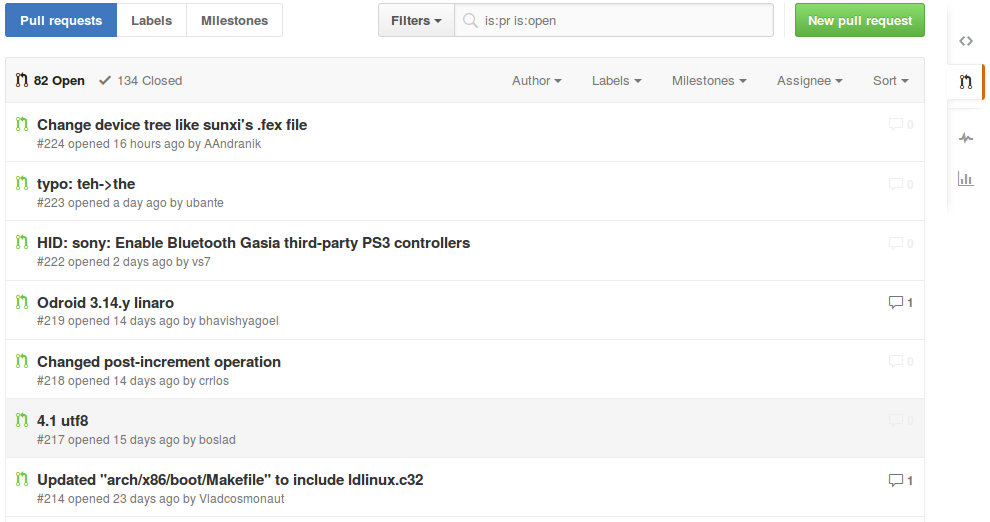
\includegraphics[width=\textwidth]{img/pull_requests_linux.png}
		\caption{Lista de pull request del kernel de Linux}
	\end{figure}
\end{frame}

\subsection{Recibir feedback}
\plain{Recibir feedback}
\begin{frame}[fragile]
	\frametitle{Discusión}

	Una vez que ha sido abierto un pull request, el equipo o persona que revisa 
	tu código puede tener dudas o comentarios.

	\pause Puede que el código no encaje con el estilo del proyecto \pause... o 
	que falten hacer pruebas unitarias \pause... o quizás está todo perfecto y 
	listo para integrar.
	\pause

	Los \textit{pull request} están diseñados para incentivar y capturar este 
	tipo de conversaciones.
\end{frame}

\subsection{Verificar}
\plain{Verificar}
\begin{frame}[fragile]
	\frametitle{Verificar los cambios en producción}

	Básicamente es probar los cambios, como si su rama fuera la rama principal.  
	En nuestro caso muy puntual sería correr el server (verificando previamente 
	que estamos en nuestra rama)

\begin{lstlisting}
$ rails s
\end{lstlisting}

	Y probar las nuevas funcionalidades que implementamos.
\end{frame}

\subsection{Mezclar}
\plain{Mezclar}
\begin{frame}[fragile]
	\frametitle{Mezclar los cambios hacia \texttt{master}}
	Luego que tus cambios han sido probados en producción, es hora de mezclar 
	tu código con la rama \texttt{master}.

	Una vez que se ha mezclado, los \textit{pull request} guardan un registro 
	de los cambios históricos a tus commits.

	\textbf{TIP:} Incorporando ciertas palabras claves en el texto de tu 
	\textit{pull request} puedes asociar incidencias al código. Cuando un 
	\textit{pull request} es mezclado, las incidencias (\textit{issues}) 
	asociadas, también son cerradas. Por ejemplo escribiendo \texttt{Closes 
		\#32} cerraría la incidencia numero 32 en el repositorio.  Para más 
	información ver 
	\href{https://help.github.com/articles/closing-issues-via-commit-messages/}{\em 
		Closing an issue in the same repository} en la ayuda de GitHub.
\end{frame}

\plain{¿Preguntas?}

\section{Bibliografía}
\begin{frame}
	\frametitle{Referencias}

	\printbibliography[heading=none]
	\nocite{*}
\end{frame}

\end{document}
